\documentclass{beamer}
% Sans animations
%\documentclass[handout]{beamer}

\usepackage{tikz}
\usetikzlibrary{calc}
\usepackage{pgfplots}
\tikzstyle{every picture}+=[remember picture]
\tikzset{
  invisible/.style={opacity=0},
  visible on/.style={alt={#1{}{invisible}}},
  alt/.code args={<#1>#2#3}{%
    \alt<#1>{\pgfkeysalso{#2}}{\pgfkeysalso{#3}} % \pgfkeysalso doesn't change the path
  },
}


\setbeamertemplate{footline}[frame number]

\title{ALG3 : récursivité et programmation dynamique}
\author{}
\date{loig.jezequel@univ-nantes.fr}

\begin{document}

\frame{
\maketitle
}

\frame{
\frametitle{Suites récursives}

\begin{block}{Suite}
Une suite est une famille d'éléments (typiquement des réels) appelés termes, indexée par les entiers naturels.
On la note en général $(u_n)$ et on note son $n$-ième terme $u_n$.
\end{block}

\begin{block}{Définition par le terme général}
On définit $u_n$ en fonction de $n$.
\end{block}

\begin{exampleblock}{Exemples}
$u_n=n$, $u_n=n!$, $u_n=1/n$, $u_n=2*n$, etc.
\end{exampleblock}

\begin{block}{Définition récursive}
On définit $u_n$ en fonction des termes précédents ($u_0, u_1, \dots, u_{n-1}$).
Dans ce cas on doit \alert{initialiser} la suite~: donner la valeur de ses premiers termes
\end{block}

\begin{exampleblock}{Exemples}
  \begin{itemize}
    \item $u_n = n\times u_{n-1}$ avec $u_0 = 1$,
    \item $u_n = u_{n-1} + u_{n-2}$ avec $u_0=0$ et $u_1=1$, etc.
  \end{itemize}
\end{exampleblock}
}

\frame{
\frametitle{Calcul itératif du $n$-ième terme d'une suite récursive simple}

\begin{block}{Suite simple}
On considère une suite $(u_n)$ telle que le terme $u_n$ ne dépend que du terme $u_{n-1}$~: $u_n = f(u_{n-1})$.
\end{block}

\begin{block}{Algorithme (calcul de $u_n$)}
Soit $i=0$ et soit $u_i = u_0$.
Tant que $i < n$, poser $u_i = f(u_i)$ puis ajouter 1 à $i$.
Retourner $u_i$.
\end{block}

\begin{exampleblock}{Exemple}
  On veut calculer $u_5$ lorsque $u_n = 2\times u_{n-1} + 1$ et $u_0 = 0$.
  \begin{enumerate}
    \item<2-> $u_i = 2\times 0 + 1 = 1$, $i = 1$
    \item<3-> $u_i = 2\times 1 + 1 = 3$, $i = 2$
    \item<4-> $u_i = 2\times 3 + 1 = 7$, $i = 3$
    \item<5-> $u_i = 2\times 7 + 1 = 15$, $i = 4$
    \item<6-> $u_i = 2\times 15 + 1 = 31$, $i = 5$
    \item<7> $i \geq 5$, on retourne $u_i = 31$
  \end{enumerate}

\end{exampleblock}
}

\frame{
\frametitle{Calcul récursif du $n$-ième terme d'une suite récursive simple}

\begin{block}{Suite simple}
On considère une suite $(u_n)$ telle que le terme $u_n$ ne dépend que du terme $u_{n-1}$~: $u_n = f(u_{n-1})$.
\end{block}

\begin{alertblock}{Fonction récursive}
  Une fonction récursive est une fonction qui s'appelle elle-même.
\end{alertblock}

\begin{block}{Algorithme (calcul récursif de $u_n$)}
  On appelle $u(i)$ la fonction qui retourne $u_0$ si $i=0$ et qui retourne $f(u(i-1))$ sinon.
  Retourner $u(n)$.
\end{block}

\begin{exampleblock}{Exemple}
On veut calculer $u_5$ lorsque $u_n = 2\times u_{n-1} + 1$ et $u_0 = 0$.

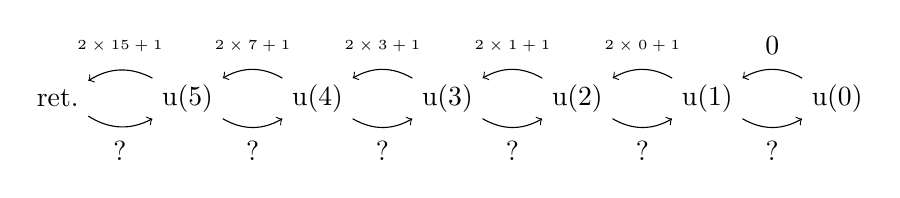
\begin{tikzpicture}[node distance=1.65cm]
  \node[visible on=<2->] (start) {ret.};
  \node[right of=start, visible on=<3->] (u5) {u(5)};
  \node[right of=u5, visible on=<4->] (u4) {u(4)};
  \node[right of=u4, visible on=<5->] (u3) {u(3)};
  \node[right of=u3, visible on=<6->] (u2) {u(2)};
  \node[right of=u2, visible on=<7->] (u1) {u(1)};
  \node[right of=u1, visible on=<8->] (u0) {u(0)};
  \path[->, visible on=<3->] (start) edge[bend right] node[yshift=-0.3cm] {?} (u5);
  \path[->, visible on=<4->] (u5) edge[bend right] node[yshift=-0.3cm] {?} (u4);
  \path[->, visible on=<5->] (u4) edge[bend right] node[yshift=-0.3cm] {?} (u3);
  \path[->, visible on=<6->] (u3) edge[bend right] node[yshift=-0.3cm] {?} (u2);
  \path[->, visible on=<7->] (u2) edge[bend right] node[yshift=-0.3cm] {?} (u1);
  \path[->, visible on=<8->] (u1) edge[bend right] node[yshift=-0.3cm] {?} (u0);
  \path[->, visible on=<9->] (u0) edge[bend right] node[yshift=0.3cm] {$0$} (u1);
  \path[->, visible on=<10->] (u1) edge[bend right] node[yshift=0.3cm] {\tiny $2\times 0 + 1$} (u2);
  \path[->, visible on=<11->] (u2) edge[bend right] node[yshift=0.3cm] {\tiny $2\times 1 + 1$} (u3);
  \path[->, visible on=<12->] (u3) edge[bend right] node[yshift=0.3cm] {\tiny $2\times 3 + 1$} (u4);
  \path[->, visible on=<13->] (u4) edge[bend right] node[yshift=0.3cm] {\tiny $2\times 7 + 1$} (u5);
  \path[->, visible on=<14->] (u5) edge[bend right] node[yshift=0.3cm] {\tiny $2\times 15 + 1$} (start);
\end{tikzpicture}
\end{exampleblock}
}

\frame{
\frametitle{À propos de la récursivité}

\begin{block}{Gros avantage}
  Les solutions à certains problèmes s'écrivent très simplement de manière récursive mais sont compliquées à écrire correctement de manière itérative (par des boucles).
\end{block}

\begin{exampleblock}{Exemple \alert{(code Go)}}
 Étant donné un tableau $t$ contenant des caractères et un entier $k\leq len(t)$, donner toutes les chaînes de $k$ caractères que l'on peut construire en utilisant au plus une fois chaque caractère de $t$.
 \begin{itemize}
   \item Pour t = \begin{tabular}{|c|c|c|c|}\hline a & b & c & d\\\hline\end{tabular} et $k=2$ on doit trouver $ab$, $ac$, $ad$, $ba$, $bc$, $bd$, $ca$, $cb$, $cd$, $da$, $db$ et $dc$.
   \item Pour t = \begin{tabular}{|c|c|c|c|}\hline a & b & c & d\\\hline\end{tabular} et $k=3$ on doit trouver $abc$, $abd$, $acb$, $acd$, $adb$, $adc$, $bac$, $bad$, $bca$, $bcd$, $bda$, $bdc$, $cab$, $cad$, $cba$, $cbd$, $cda$, $cdb$, $dab$, $dac$, $dba$, $dbc$, $dca$, $dcb$.
 \end{itemize}
\end{exampleblock}

\begin{exampleblock}{Autres exemples plus tard}
Tri fusion, algorithmes sur les arbres
\end{exampleblock}
}

\frame{
\frametitle{À propos de la récursivité, suite}

\begin{block}{Soyez prudents}
  \begin{itemize}
    \item Un appel de fonction est plus long qu'un tour de boucle.
    \item Les appels de fonctions non résolus occupent la mémoire.
  \end{itemize}
\end{block}

\begin{block}{Récursivité terminale}
Si l'appel récursif est la dernière chose qui se passe dans une fonction, le compilateur peut optimiser et éviter les appels de fonctions non résolus.
\end{block}

\begin{block}{Remarque}
Une fonction récursive peut toujours être rendue récursive terminale en utilisant la notion de continuation.
Cependant, c'est un peu compliqué et on n'en parlera pas dans ce cours.
\end{block}
}

\frame{
\frametitle{Un exemple un peu plus compliqué~: la suite de Fibonacci}

\begin{block}{Histoire}
Cette suite est tirée d'un problème proposé en 1202 par le mathématicien italien Fibonacci, mais elle avait été étudiée avant par les mathématiciens indiens pour résoudre d'autres problèmes.
\end{block}

\begin{block}{Définition d'origine}
Quelqu’un a déposé un couple de lapins dans un certain lieu, clos de toutes parts, pour savoir combien de couples seraient issus de cette paire en une année, car il est dans leur nature de générer un autre couple en un seul mois, et qu’ils enfantent dans le second mois après leur naissance.
\end{block}

\begin{block}{Définition sous forme de suite}
La suite de Fibonacci est la suite $(u_n)$ telle que $u_n = u_{n-1} + u_{n-2}$ avec $u_0 = 0$ et $u_1 = 1$.
\end{block}

}

\frame{
\frametitle{La suite de Fibonacci, suite}

\begin{block}{Implantation naïve \alert{(code Go)}}
Si on calcule simplement le $n$-ième terme de cette suite en appliquant la définition récursive, ce n'est pas très efficace.
\end{block}

\pause

\begin{block}{Arbre des appels récursifs}
On peut comprendre pourquoi en représentant l'arbre des appels récursifs correspondant (ici pour le calcul de $f(5)$).

\begin{center}
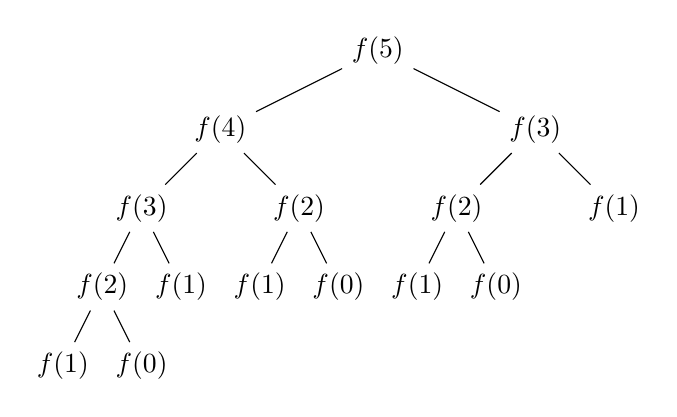
\begin{tikzpicture}[node distance=1cm]
  \node (31) {$f(2)$};
  \node[right of=31] (32) {$f(1)$};
  \node[right of=32] (33) {$f(1)$};
  \node[right of=33] (34) {$f(0)$};
  \node[right of=34] (35) {$f(1)$};
  \node[right of=35] (36) {$f(0)$};
  \node (tmp) at ($(31)!0.5!(32)$) {};
  \node[above of=tmp] (21) {$f(3)$};
  \node[right of=21] (tmp) {};
  \node[right of=tmp] (22) {$f(2)$};
  \node[right of=22] (tmp) {};
  \node[right of=tmp] (23) {$f(2)$};
  \node[right of=23] (tmp) {};
  \node[right of=tmp] (24) {$f(1)$};
  \node (tmp) at ($(21)!0.5!(22)$) {};
  \node[above of=tmp] (11) {$f(4)$};
  \node (tmp) at ($(23)!0.5!(24)$) {};
  \node[above of=tmp] (12) {$f(3)$};
  \node (tmp) at ($(11)!0.5!(12)$) {};
  \node[above of=tmp] (0) {$f(5)$};
  \node (tmp) at ($(31)!0.5!(32)$) {};
  \node[below of=tmp] (42) {$f(0)$};
  \node[left of=42] (41) {$f(1)$};
  \path (0)  edge (11)
             edge (12)
        (11) edge (21)
             edge (22)
        (12) edge (23)
             edge (24)
        (21) edge (31)
             edge (32)
        (22) edge (33)
             edge (34)
        (23) edge (35)
             edge (36)
        (31) edge (41)
             edge (42);
\end{tikzpicture}
\end{center}
\end{block}

}

\frame{
\frametitle{La suite de Fibonacci, le retour}

\begin{block}{Programmation dynamique}
Dans une telle situation, on peut éviter les appels récursifs redondants en stockant dans un tableau la valeur obtenue lors du premier appel et en la récupérant lors des appels suivants.
\end{block}

\begin{block}{Arbre des appels récursifs et des accès au tableau \alert{(code Go)}}
\begin{center}
\begin{tikzpicture}[node distance=0.8cm]
  \node (31) {$f(2)$};
  \node[right of=31] (32) {$t(1)$};
  \node[right of=32] (33) {};
  \node[right of=33] (34) {};
  \node[right of=34] (35) {};
  \node[right of=35] (36) {};
  \node (tmp) at ($(31)!0.5!(32)$) {};
  \node[above of=tmp] (21) {$f(3)$};
  \node[right of=21] (tmp) {};
  \node[right of=tmp] (22) {$t(2)$};
  \node[right of=22] (tmp) {};
  \node[right of=tmp] (23) {};
  \node[right of=23] (tmp) {};
  \node[right of=tmp] (24) {};
  \node (tmp) at ($(21)!0.5!(22)$) {};
  \node[above of=tmp] (11) {$f(4)$};
  \node (tmp) at ($(23)!0.5!(24)$) {};
  \node[above of=tmp] (12) {$t(3)$};
  \node (tmp) at ($(11)!0.5!(12)$) {};
  \node[above of=tmp] (0) {$f(5)$};
  \node (tmp) at ($(31)!0.5!(32)$) {};
  \node[below of=tmp] (42) {$t(0)$};
  \node[left of=42] (41) {$t(1)$};
  \path (0)  edge (11)
             edge (12)
        (11) edge (21)
             edge (22)
        (21) edge (31)
             edge (32)
        (31) edge (41)
             edge (42);
\end{tikzpicture}
\end{center}
Il existe aussi une version sans tableau (qui ne stocke que deux valeurs à chaque instant) et récursive terminale. \alert{(code Go)}
\end{block}

}

\frame{
\frametitle{Un exemple plus compliqué de programmation dynamique}

\begin{block}{Sous-chaînes}
Étant donnée une chaîne de caractères $s$ on appelle sous-chaîne de $s$ toute chaîne de caractères $s'$ telle que $len(s')\leq len(s)$ et telle qu'il existe des entiers $i_0<i_1<\dots<i_{len(s')-1}$ tels que quel que soit $0\leq j<len(s')$ on a $0\leq i_j < len(s)$ et $s'[j]=s[i_j]$.
\end{block}

\begin{exampleblock}{Exemples}
$bisou$, $ours$, $bison$, $bonus$, $sono$, et $iso$ sont des quelques-unes des sous-chaînes de $bisounours$.
\end{exampleblock}

\begin{block}{Problème de la plus longue sous-chaîne commune}
Étant données deux chaînes de caractères $s_1$ et $s_2$, trouver la plus longue sous-chaîne de $s_1$ qui est aussi une sous-chaîne de $s_2$.
\end{block}

\begin{exampleblock}{Exemple}
Les sous-chaînes communes de $bisounours$ et $souris$ sont
$s$, $o$, $u$, $r$, $i$,
$so$, $su$, $sr$, $ss$,
$ou$, $or$, $os$,
$ur$, $us$,
$rs$,
$is$,
$sou$, $sor$, $sos$,
$sur$, $sus$,
$srs$,
$our$, $ous$,
$ors$,
$urs$,
$sour$, $sous$,
$ours$, et
$sours$.
La plus longue est $sours$.
\end{exampleblock}

}

\frame{
\frametitle{Sous-chaînes et force brute}

\begin{block}{Première approche}
Pour résoudre le problème on pourrait calculer toutes les sous-chaînes de $s_1$, puis vérifier une-à-une (en commençant par la plus grande) si ce sont des sous-chaînes de $s_2$.
\end{block}

\begin{block}{Nombre de sous-chaînes}
Une chaîne de caractères $s$ de longueur $n$ a jusqu'à $2^n$ sous-chaînes.
\end{block}

\begin{block}{Vérifier qu'une sous-chaîne est contenue dans une chaîne}
Étant données une chaîne $s$ et une chaîne $s'$, vérifier que $s'$ est une sous chaîne de $s$ peut impliquer de regarder un à un tous les caractères de $s$.
\end{block}

\begin{block}{Ordre de grandeur du nombre d'opérations dans le pire cas}
Si $s_1$ a pour longueur $n$ et $s_2$ a pour longueur $m$, on fera de l'ordre de $2^n\times m$ opérations pour résoudre le problème.
\end{block}

}

\frame{
\frametitle{Sous-chaînes, version récursive}

\begin{block}{Remarques fondamentales}
  Soient $s_1'$ et $s_2'$ des chaînes de caractères, soient $c_1$ et $c_2$ des caractères et soit $s$ une plus grande sous-chaîne commune à $s_1=s_1'c_1$ et $s_2=s_2'c_2$.
\begin{itemize}
\item Si $c_1 = c_2$ alors $s = s'c_1$ avec $s'$ une plus grande sous-chaîne commune à $s_1'$ et $s_2'$.
\item Si $c_1 \neq c_2$ alors $s$ est une plus grande sous-chaîne commune à $s_1$ et $s_2'$ ou à $s_1'$ et $s_2$.
\end{itemize}
\end{block}

\begin{block}{Définition récursive d'une plus grande sous-chaîne commune}
  \vspace*{-0.5cm}
$$sc(s_1, s_2) = \left\{ \begin{array}{ll}
\varepsilon & \texttt{si } len(s_1) = 0 \texttt{ ou } len(s_2)=0 \\
sc(s_1',s_2')c & \texttt{si } s_1=s_1'c \texttt{ et } s_2 = s_2'c\\
sc(s_1',s_2) & \texttt{si } s_1=s_1'c_1, s_2=s_2'c_2 \texttt{ avec } c_1\neq c_2 \\
             & \texttt{et } len(sc(s_1',s_2)) \geq len(sc(s_1, s_2')) \\
sc(s_1,s_2') & \texttt{si } s_1=s_1'c_1, s_2=s_2'c_2 \texttt{ avec } c_1\neq c_2 \\
             & \texttt{et } len(sc(s_1',s_2)) < len(sc(s_1, s_2'))
\end{array}\right.$$
\end{block}

}

\frame{
\frametitle{Plus grande sous-chaîne et programmation dynamique}

\begin{exampleblock}{Exemple d'arbre des appels récursifs pour $s_1 = ab$ et $s_2 = bcd$}

\begin{center}
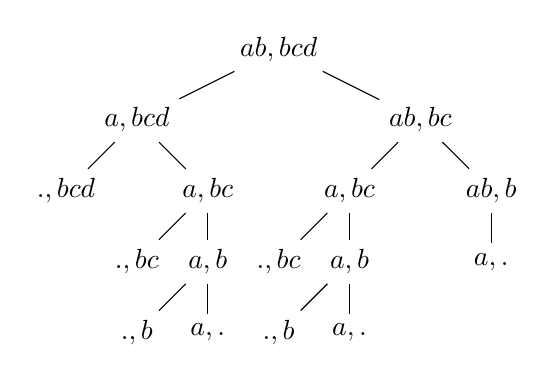
\begin{tikzpicture}[node distance=0.9cm]
  \node (tmp) {};
  \node[left of=tmp] (tmp1) {};
  \node[left of=tmp1] (11) {$ab,bcd$};
  \node[below of=11] (tmp) {};
  \node[left of=tmp] (tmp1) {};
  \node[left of=tmp1] (21) {$a,bcd$};
  \node[right of=tmp] (tmp2) {};
  \node[right of=tmp2] (22) {$ab,bc$};
  \node[below of=21] (tmp) {};
  \node[left of=tmp] (31) {$.,bcd$};
  \node[right of=tmp] (32) {$a,bc$};
  \node[below of=tmp] (41) {$.,bc$};
  \node[right of=41] (42) {$a,b$};
  \node[below of=22] (tmp) {};
  \node[left of=tmp] (33) {$a,bc$};
  \node[right of=tmp] (34) {$ab,b$};
  \node[right of=42] (43) {$.,bc$};
  \node[right of=43] (44) {$a,b$};
  \node[below of=34] (45) {$a,.$};
  \node[below of=41] (51) {$.,b$};
  \node[right of=51] (52) {$a,.$};
  \node[right of=52] (53) {$.,b$};
  \node[right of=53] (54) {$a,.$};
  \path (11) edge (21)
             edge (22)
        (21) edge (31)
             edge (32)
        (22) edge (33)
             edge (34)
        (32) edge (41)
             edge (42)
        (33) edge (43)
             edge (44)
        (34) edge (45)
        (42) edge (51)
             edge (52)
        (44) edge (53)
             edge (54);
\end{tikzpicture}
\end{center}
\end{exampleblock}

\begin{block}{Réduire les appels récursifs \alert{(code Go)}}
  Utilisation d'un tableau $t$ à deux dimensions, la case $t[i][j]$ indique la solution du problème pour les chaînes constituées des $i$ premiers caractères de $s_1$ et des $j$ premiers caractères de $s_2$.
\end{block}
}

\frame{
\frametitle{Plus grande sous-chaîne et nombres d'opérations}

%\begin{block}{Ordres de grandeur des nombres d'opérations dans le pire cas}
  On considère que $len(s_1) = n \leq len(s_2) = m$.
\begin{description}
\item[Force brute~:] de l'ordre de $2^n\times m$ opérations
\item[Récursivité~:] de l'ordre de $n\times m$ opérations (remplir le tableau $t$)
\end{description}
%\end{block}

\begin{center}
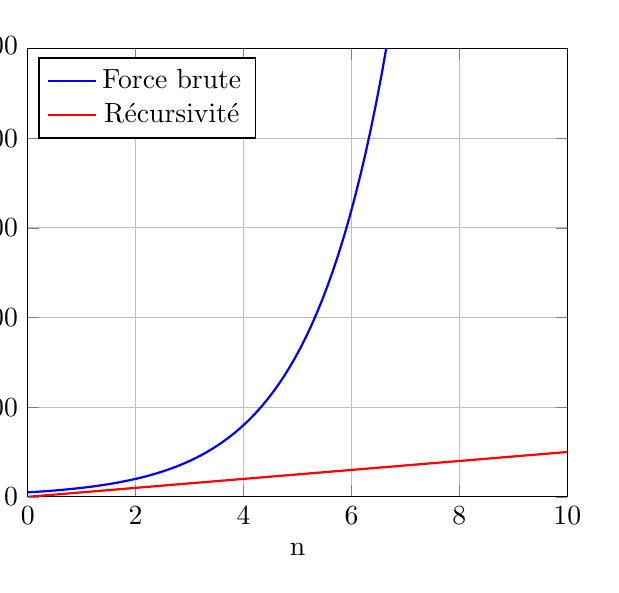
\begin{tikzpicture}[trim axis left]
\begin{axis}[domain=0:10,
  samples=100,
  enlarge x limits=false,
  grid=both,
  no markers,
  ymin=0., ymax=1000.,
  xmin=0., xmax=10.,
  xlabel={n},
  ylabel={nombre d'opérations pour $m=10$},
  legend style={at={(0.02,0.98)}, anchor=north west}]
\addplot +[thick] {2^x*10};
\addlegendentry{Force brute}
\addplot +[thick] {x*10};
\addlegendentry{Récursivité}
\end{axis}
\end{tikzpicture}
\end{center}
}

\frame{
\frametitle{Quand utiliser la programmation dynamique pour résoudre un problème ?}

\begin{block}{Sous-problèmes de même nature}
Si on peut \alert{résoudre} le problème \alert{en combinant les solutions de plusieurs problèmes plus petits} mais de même nature que le problème d'origine (qui peuvent se résoudre de la même façon, en appliquant le même algorithme) alors on pourra le résoudre récursivement.
\end{block}

\begin{block}{Chevauchement des sous-problèmes}
Si le nombre de sous-problèmes différents résolus au cours d'une résolution récursive du problème et petit par rapport au nombres de sous-problèmes résolus, donc si on \alert{résout souvent les mêmes sous-problèmes}, on pourra améliorer les performances grace à la programmation dynamique.
\end{block}

}

\end{document}
